\documentclass[french, 11pt]{article}

%-------------------------------------------------------------------------------
\usepackage[a4paper,top=1cm,bottom=2cm,left=1cm,right=1cm,marginparwidth=0.5cm]{geometry}
\usepackage{amsmath,amsfonts,amssymb,amsthm}
\usepackage[french]{babel}
\usepackage[utf8]{inputenc}
\usepackage[T1]{fontenc}
\usepackage{enumerate}
\usepackage{natbib}
\usepackage{graphicx}
\usepackage{xspace}
\usepackage{color,xcolor}
\usepackage{tikz}
\usepackage{remreset}
\usepackage{url}
\usepackage{boites}
% \usepackage{extsizes} % Permet \documentclass[french, 14pt]{extreport}
% \usepackage[a4paper,top=1cm,bottom=2cm,left=1cm,right=1cm,marginparwidth=.75cm]{geometry}
% \usepackage{minitoc}

\graphicspath{{../Figures/}}
% Environnement
\newtheorem{theorem}{Théorème}
\newtheorem{definition}{Définition}
\newtheorem{lemma}{Lemme}
\newtheorem{proposition}{Proposition}
\newtheorem*{theorem*}{Théorème}
\newtheorem*{definition*}{Définition}
\newtheorem*{proposition*}{Proposition}
\newtheorem*{corollary*}{Corollaire}
\newtheorem*{assumption*}{Hypothèse}
\newtheorem*{algorithm*}{Algorithme}
\newtheorem*{lemma*}{Lemme}
\newtheorem*{remark*}{Remarque}
\newtheorem*{exercise*}{Exercice}
\newtheorem{exercise}{Exercice}
\newcommand{\remark}{\bigskip\noindent\textbf{\textsl{Remarque.}}\xspace}
\newcommand{\remarks}{\bigskip\noindent\textbf{\textsl{Remarques.}}\xspace}
\newcommand{\parSR}[1]{\paragraph*{\textsl{#1}}\xspace}
\renewcommand{\proof}{\bigskip\noindent\underline{\textsl{Démonstration}.}\xspace}
\newcommand{\eproof}{$\blacksquare$}

% Effets, couleurs
\newcommand{\emphase}[1]{\textcolor{red}{#1}}
\newcommand{\demoProp}[1]{\noindent{\textbf{\textsl{Démonstration de la proposition \ref{#1} :}}}}
\newcommand{\itemdot}{\textbullet}

% Moments
\DeclareMathOperator{\Esp}{\mathbb{E}}
\DeclareMathOperator{\diag}{diag}
\DeclareMathOperator{\Cov}{\mathbb{C}ov}
\DeclareMathOperator{\tr}{tr}
\DeclareMathOperator{\Var}{\mathbb{V}}
\let\Pr\relax\DeclareMathOperator{\Pr}{\mathbb{P}}
\renewcommand{\d}{\text{d}}

% R, N, ...
\newcommand{\cst}{\text{cst}}
\newcommand{\Cbb}{\mathbb{C}}
\newcommand{\Ibb}{\mathbb{I}}
\newcommand{\Nbb}{\mathbb{N}}
\newcommand{\Rbb}{\mathbb{R}}
\newcommand{\Zbb}{\mathbb{Z}}

% Indicateurs

% Lois et ensembles
\newcommand{\Acal}{\mathcal{A}}
\newcommand{\Bcal}{\mathcal{B}}
\newcommand{\Ccal}{\mathcal{C}}
\newcommand{\Ecal}{\mathcal{E}}
\newcommand{\Gcal}{\mathcal{G}}
\newcommand{\Ical}{\mathcal{I}}
\newcommand{\Lcal}{\mathcal{L}}
\newcommand{\Mcal}{\mathcal{M}}
\newcommand{\Ncal}{\mathcal{N}}
\newcommand{\Pcal}{\mathcal{P}}
\newcommand{\Rcal}{\mathcal{R}}
\newcommand{\Scal}{\mathcal{S}}
\newcommand{\Ucal}{\mathcal{U}}
\newcommand{\Xcal}{\mathcal{X}}
\newcommand{\Ycal}{\mathcal{Y}}

% Comments
\newcommand{\SR}[2]{\textcolor{gray}{#1}\textcolor{red}{#2}}
\newcommand{\todo}[1]{\textcolor{red}{\`A faire~: {\sl #1}}}
\newcommand{\dessin}[1]{
\begin{center}\framebox{\begin{minipage}{\textwidth}
  \textcolor{purple}{#1}
\end{minipage}}\end{center}
\bigskip
}
\newcommand{\progres}[1]{
\begin{center}\framebox{\begin{minipage}{\textwidth}
  \textcolor{blue}{{\sl #1}}
\end{minipage}}\end{center}
\bigskip
}
\newcommand{\solution}[1]{
\begin{center}\framebox{\begin{minipage}{\textwidth}
  \noindent{\sl Solution :}
  #1
\end{minipage}}\end{center}
\bigskip
}
% \newcommand{\exemple}[1]{
% \begin{center}\framebox{\begin{minipage}{\textwidth}
%   \parSR{Exemple.}
%   #1
% \end{minipage}}\end{center}
% \bigskip
% }
\newcommand{\exemple}[1]{
\begin{breakbox}
  \parSR{Exemple.}
  #1
\end{breakbox}
\bigskip
}

\newcommand{\SRcorrect}[2]{\textcolor{gray}{#1}\textcolor{blue}{#2}}
\newcommand{\SRcomment}[1]{\textcolor{blue}{[{\sl SR: #1}]}}



% Section numbering
\usepackage{chngcntr}
\renewcommand{\thepart}{\Roman{part}}
% \counterwithout{section}{part}
\setcounter{secnumdepth}{3}
\setcounter{tocdepth}{1}

% Proposition numbering
\renewcommand{\subsubsection}{\section}
% \numberwithin{exercise}{section}
% \numberwithin{equation}{section}

% Suppression des solutions
\renewcommand{\solution}[1]{}

\newcommand{\alglin}{/home/robin/ENSEIGN/Cours/MathBiologie/L3-ENS-Math1/Exercices/AlgLin}
\newcommand{\multivar}{/home/robin/ENSEIGN/Cours/MathBiologie/L3-ENS-Math1/Exercices/MultiVar}
\newcommand{\equadiff}{/home/robin/ENSEIGN/Cours/MathBiologie/L3-ENS-Math1/Exercices/EquaDiff}
\newcommand{\probas}{/home/robin/ENSEIGN/Cours/MathBiologie/L3-ENS-Math1/Exercices/Probas}


% %-------------------------------------------------------------------------------
% %-------------------------------------------------------------------------------
% \title{\Huge{Ce qu'un biologiste doit savoir en mathématiques}}
% \author{SR d'après \cite{Lam20} : Annexes}
% \date{\today}


\title{\normalsize{\sc École Normale Supérieure de Paris, Licence de Biologie L3}
  
  \bigskip
  \normalsize{\sc Année 2025–26}
  
  \bigskip
  \large{\bf Mathématiques I : ce qu’un biologiste ne doit pas ignorer} 
  
}
\date{Examen, le 16 janvier 2026}

%-------------------------------------------------------------------------------
%-------------------------------------------------------------------------------
\begin{document}
%-------------------------------------------------------------------------------
%-------------------------------------------------------------------------------

\maketitle

\bigskip
L'épreuve dure 2 heures. 
Les notes de cours individuelles sont autorisées.
L’usage de tout appareil électronique est interdit à l’exception d’une calculatrice.

%-------------------------------------------------------------------------------
% \section{Algèbre linéaire}
% \input{\alglin/}

%-------------------------------------------------------------------------------
% \section{Fonction de plusieurs variables}
%-------------------------------------------------------------------------------
\subsubsection{Application linéaire tangente à une forme quadratique} 
%-------------------------------------------------------------------------------

On considère une matrice $A \in \Mcal_n$ symétrique, un vecteur $v \in \Rbb^n$ et la fonction 
$$
\begin{array}{rlll}
  f : & \Rbb^n & \mapsto & \Rbb \\
  & x & \to & f(x) = x^\top A x + v^\top x.
\end{array}
$$

\begin{enumerate}
  \item Montrer qu'il existe un vecteur $g(x) \in \Rbb^n$, qu'on précisera, tel que l'application linéaire tangente à $f$ en $x$ s'écrit
  $$
  \begin{array}{rlll}
    D_xf : & \Rbb^n & \mapsto & \Rbb^n \\
    & h & \to & D_xf(h) = g(x)^\top h.
  \end{array}
  $$
  \solution{On écrit
  \begin{align*}
    f(x+h) 
    & = (x+h)^\top A (x+h) + v^\top (x+h)
    = f(x) + x^\top A h + h^\top A x + h^\top A h + v^\top h \\
    & = f(x) + (2 x^\top A + v^\top) h + h^\top A h
  \end{align*}
  puisque $x^\top A h = h^\top A x$. On remarque alors que $h^\top A h = o(\|h\|)$ pour conclure que, puisque $A$ est symétrique, l'application linéaire tangent $D_x f$ s'écrit bien
  $$
  D_xf(h) = g(x)^\top h
  \qquad \text{avec} \quad
  g(x) = 2 A x + v.
  $$}
  \item En supposant que $A$ est inversible, déterminer le point stationnaire $x^*$ où $g(x)$ s'annule.
  \solution{En supposant $A$ inversible, on a
  $$
  g(x^*) = 0
  \qquad \Leftrightarrow \qquad
  2 A x^* + v = 0
  \qquad \Leftrightarrow \qquad
  x^* = - \frac12 A^{-1} v.
  $$}
  \item Donner une condition sur$A$ pour que $A$ soit un minimum local. (On pourra calculer la matrice hessienne de $A$.)
  \solution{La matrice hessienne de l'application $f$ en tout point $x$ vaut $H_x = 2 A$ (il suffit de déterminer l'application linéaire tangente à $g(x)$).
  $x^*$ est donc un minimum ssi $A$ est strictement définie négative}
  \item Discuter l'utilité de l'hypothèse selon laquelle $A$ est symétrique.
  \solution{On peut décomposer $A$ en ses parties symétrique $S$ et anti-symétrique $T$ : 
  $$
  S = \frac12(A + A^\top), \qquad 
  T = \frac12(A - A^\top), \qquad 
  \Rightarrow \quad
  A = S + T
  $$
  et remarquer que
  $$
  f(x) 
  = x^\top A x + v^\top x
  = x^\top S x + \frac12 \underset{=0}{\underbrace{(x^\top A x - x^\top A^\top x)}} + v^\top x,  
  $$
  c'est-à-dire que seulle la partie symétrique de $A$ contribue à la fonction Ode $f$.}
\end{enumerate}




%-------------------------------------------------------------------------------
% \section{Systèmes dynamiques}
%-------------------------------------------------------------------------------
\subsubsection{Dynamique de population à trois classes : mâles, femelles et couples}
%-------------------------------------------------------------------------------

On considère une population sexuée panmictique, au sein de laquelle on désigne
respectivement par $x(t)$, $y(t)$ et $z(t)$ les densités au temps $t$ de femelles flottantes, de mâles flottants, et de couples. On suppose que la dynamique de la population respecte le système dynamique suivant
\begin{equation} \label{eq:Dyn3Pop}
  \left\{\begin{array}{rcl}
          \dot x(t) & = & - \alpha x y + r z, \\
          \dot y(t) & = & - \alpha x y + r z, \\
          \dot z(t) & = & + \alpha x y - c z^2,
          \end{array} \right.
\end{equation}
où les coefficients $\alpha$, $r$ et $c$ sont strictement positifs.
\begin{enumerate}
  \item Interpréter ces équations et la signification de chacun des coefficients $\alpha$, $r$ et $c$.
  \solution{Les mâles et femelles flottant(e)s s'apparient pour former des couples : 
  \begin{itemize}
    \item $\alpha$ est le taux de formation des couples, 
    \item $r$ est le taux de natalités de mâles et des femelles (supposés égaux),
    \item $c$ est le taux de mortalité des couples.
  \end{itemize}
  }
  \item En notant $S = x(0) - y(0)$, montrer que $x(t) - y(t) = S$ pour tout temps $t$. En
  déduire les fonctions $y$ et $z$ satisfont le système 
  \begin{equation} \label{eq:Dyn3Pop2}
    \left\{\begin{array}{rcl}
            \dot y(t) & = & - \alpha (y^2 + Sy) + r z, \\
            \dot z(t) & = & + \alpha (y^2 + Sy) - c z^2.
            \end{array} \right.
  \end{equation}
  Dans la suite on supposera que $S > 0$.
  \solution{On remarque que
  $$
  \dot x(t) - \dot y(t) = 0,
  $$
  ce qui implique que la différence $x(t) - y(t)$ reste constante au cours du temps et égale à $x(0) - y(0) = S$. \\
  On peut donc remplacer $x(t) = y(t) + S$ dans le système \eqref{eq:Dyn3Pop} pour obtenir le système \eqref{eq:Dyn3Pop2}.}
  \item Déterminer les points d'équilibre du système \eqref{eq:Dyn3Pop2}.
  \solution{
  \begin{itemize}
    \item $(y^* = 0, z^* = 0)$ est un équilibre (trivial).
    \item $(y = -S, z^* = 0)$ n'est pas un équilibre intéressant du point de vue du modèle car on s'intéresse aux effectifs positifs ou nuls. 
    \item Si on suppose $({y^*}^2 + Sy^*) \neq 0$, il vient
    $$
    \alpha({y^*}^2 + Sy^*) = rz^* = c{z^*}^2 
    \qquad \Rightarrow \qquad 
    z^* = r / c
    $$
    et $y^*$ doit vérifier
    $$
    {y^*}^2 + Sy^* - \frac{r^2}{\alpha c} = 0,
    $$
    dont le discriminant est 
    $$
    \Delta =  S^2 + \frac{4 r^2}{\alpha c} > S^2,
    $$
    et dont la seule solution positive est
    $$
    y^* = \frac{\sqrt{\Delta} - S}2.
    $$
    Le second équilibre intéressant est donc $(y^* = (\sqrt{\Delta} - S)/2, z^* = r/c)$. \\
    $(y^* = (-\sqrt{\Delta} - S)/2, z^* = r/c)$ est bien un point d'équilibre, mais sans intérêt du point de vue du modèle.
  \end{itemize}
  }
  \item \'Ecrire la matrice jacobienne du système \eqref{eq:Dyn3Pop2} et étudier la nature du ou des équilibres non triviaux.
  \solution{La jacobienne vaut
  $$
  J = \left[\begin{array}{rr}
              -2 \alpha y - \alpha S & r \\ 2 \alpha y + \alpha S & -2 c z
            \end{array}\right]
  $$
  \begin{description}
    \item[En $(0, 0)$ :] on a 
    $$
    J_{(0, 0)} = \left[\begin{array}{rr}
                - \alpha S & r \\ \alpha S & 0
              \end{array}\right]
    \qquad \Rightarrow \qquad
    P(\lambda) = \lambda^2 + \alpha S \lambda - r \alpha S
    $$
    où
    $$
    \Delta_0 = \alpha^2 S^2 (1 - 4 r / (\alpha S)).
    $$
    \begin{itemize}
      \item Si $\Delta_0 \geq 0$, les deux valeurs propres
      $$
      \lambda = \frac{\alpha S}2 \left(-1 \pm \sqrt{1 - 4r/(\alpha S)}\right)
      $$
      sont négatives (car $\sqrt{1 - 4r/(\alpha S)} < 1$) et $(0, 0)$ est un équilibre stable. 
      \item Si $\Delta_0 < 0$, la partie réelle ($-\alpha S/2$) des deux valeurs propres est négative et l'équilibre est également stable.
    \end{itemize}
    \item[En $(y^* = \sqrt{\Delta} - S)/2, z^* = r/c)$ :] on a 
    $$
    J_{(y^*, z^*)} = \left[\begin{array}{rr}
                - \alpha \delta & r \\ \alpha \delta & -2 r
              \end{array}\right]
    \qquad \Rightarrow \qquad
    P(\lambda) = \lambda^2 + (\alpha \delta + 2r) \lambda - r \alpha \delta,
    $$
    en notant $\delta = 2(\sqrt{\Delta} - S) + S = 2\sqrt{\Delta} - S > 0$. On a cette fois
    $$
    \Delta^* 
    = \frac12 \left((\alpha \delta + 2r)^2 - 4 r \alpha \delta\right)
    = \frac12 (\alpha \delta - 2r)^2 \geq 0,
    $$
    soit
    $$
    \lambda = \frac12 \left(-(\alpha \delta + 2r) \pm \sqrt{\Delta^* }\right) \leq 0
    $$
    car, les coefficients $\alpha$, $r$ et $c$ étant tous positifs,
    $$
    \frac12 (\alpha \delta - 2r)^2 < (\alpha \delta + 2r)^2.
    $$
    $(y^* = \sqrt{\Delta} - S)/2, z^* = r/c)$ est donc un équilibre stable.
    
  \end{description}
  $$
  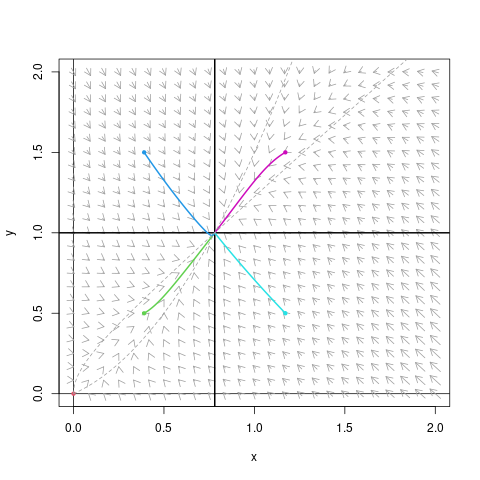
\includegraphics[width=.5\textwidth]{DynPopMaleFemelleCouple.png}
  $$
  }
\end{enumerate}



%-------------------------------------------------------------------------------
% \section{Probabilités}
%-------------------------------------------------------------------------------
\subsubsection{Chaîne de Markov à deux états absorbants}
%-------------------------------------------------------------------------------

On considère une chaîne de Markov $(X_n)_{n \geq 0}$ prenant ses valeurs dans $\{0, \dots \ell\}$, et on note $p_{i, j}$ la probabilité de transition de de l'état $i$ vers l'état $j$. On suppose que 
$$
p_{0, 0} = p_{\ell, \ell} = 1 
$$
et que, pour tout $1 \leq i, j \leq \ell-1$, 
$$
p_{i, 0} = a > 0, \qquad p_{i, \ell} = b > 0, \qquad p_{i, j} \geq 0.
$$
On note de plus $T_{i, j}$ le temps d'atteinte de l'état $j$ à partir de l'état $i$:
$$
T_{i, j} = \min\{n: X_n = j \mid X_0 = i\}.
$$

\begin{enumerate}
  \item Donner la matrice de transition et tracer le graphe de transition de cette chaîne de Markov.
  \solution{
  $$
  P = \left(\begin{array}{c|ccc|c}
              1 & 0 & \cdots & 0 & 0 \\
              \hline
              a & p_{2, 2} & \cdots & p_{2, a-1} & b \\
              \vdots & \vdots &  & \vdots & \vdots \\
              a & p_{a-1, 2} & \cdots & p_{a-1, a-1} & b \\
              \hline
              0 & 0 & \cdots & 0 & 1
          \end{array}\right).
  $$}
  \item Quelles sont les classes de communication de cette chaîne ? Donner leur nature. Quels sont les comportements asymptotiques possibles de cette chaîne ?
  \solution{Les classes de communications sont 
  $$
  C_1 = \{0\}, \qquad C_2 = \{1, \dots, \ell-1\}, \qquad C_3 = \{\ell\}.
  $$
  $C_1$ et $C_3$ sont absorbantes, $C_2$ est transiente. La chaîne finit nécessairement par être absorbé en 0 ou $\ell$.}
  \item Soit $1 \leq i \leq \ell-1$, donner la probabilité que $X_{n+1} \in \{1, \dots \ell-1\}$ sachant que $X_n = i$.
  \solution{Pour tout $1 \leq i \leq \ell-1$, on a $p_{i, 0} = a$ et $p_{i, \ell} = b$, donc
  $$
  \Pr\{1 \leq X_{n+1} \leq \ell-1 \mid X_n = i\}
  = \Pr\{X_{n+1} \neq 0 \text{ et } X_{n+1} \neq \ell\}
  = 1 -(a+b).
  $$}
  \item En déduire que, pour $1 \leq i \leq \ell-1$, en notant $c = a + b$, 
  $$
  \Pr\{T_{i, 0} = n\} = a (1 - c)^{n-1}, \qquad
  \Pr\{T_{i, \ell} = n\} = b (1 - c)^{n-1}.
  $$
  \solution{A chaque pas de temps, partant d'un état $1 \leq i \leq \ell-1$, la chaîne reste dans $\{1, \dots, \ell-1\}$ avec probabilité $1 - a - b = 1 - c$ et passe dans l'état 0 avec probabilité $a$. Pour atteindre l'état 0 depuis l'état $i$ en $n$ étapes, la chaîne doit rester $n-1$ fois dans $\{1, \dots, \ell-1\}$ (avec probabilité $(1-c)^{n-1}$) puis passer en 0 (avec probabilité $a$). \\
  L'autre résultat s'obtient par symétrie}
  \item Pour $1 \leq i \leq \ell-1$, on note maintenant $T_i$ le temps d’absorption (en 0 ou en $\ell$) : 
  $$
  T_i = \min(T_{i, 0}, T_{i, \ell}).
  $$
  Montrer que $T_i$ suit une loi géométrique $\Gcal(c)$ : $\Pr\{T_i = n\} = c (1 - c)^{n-1}$. \\
  En déduire son espérance.
  \solution{Il suffit de remarquer que l'événement d'absorption au temps $n$ s'écrit
  $$
  \{X_n \in \{0, \ell\}, X_0 = i\} = \{X_n = 0, X_0 = i\} \cup \{X_n = \ell, X_0 = i\}
  $$
  pour en déduire que 
  $$
  \Pr\{T_i = n\} = \Pr\{T_{i, 0} = n\} + \Pr\{T_{i, \ell} = n\} = (a + b) (1 - c)^{n-1}.
  $$
  De plus, en se souvenant que 
  $$
  \sum_{n \geq 1} n x^{n-1} 
  = \partial_x \sum_{n \geq 0} x^n 
  = \partial_x \frac{1}{1 - x}
  = (1 - x)^{-2}, 
  $$
  on obtient
  $$
  \Esp T_i = \sum_{n \geq 1} n c (1 - c)^{n-1} = c (1 - (1-c))^{-2} = 1/c.
  $$}
%   \item Montrer que, pour $1 \leq i \leq \ell-1$, 
%   $$
%   \Pr\{T_{i, 0} < n\} = \frac{a [1 - (1 - c)^{n-1}]}{c}.
%   $$
%   \solution{
%   \begin{align*}
%   \Pr\{T_{i, 0} < n\} 
%   & = \sum_{m =1}^{n-1} \Pr\{T_{i, 0} = m \} 
%   = a \sum_{m = 1}^{n-1} (1 - c)^{m-1} \\
%   & = \frac{a [1 - (1 - c)^{n-1}]}{1 - (1 - c)} 
%   = \frac{a [1 - (1 - c)^{n-1}]}{c}.
%   \end{align*}}
  \item Pour $1 \leq i \leq \ell-1$, calculer la probabilité que, partant de $X_0 = i$ la chaîne de Markov atteigne l'état 0 avant l'état $\ell$.
  \solution{La chaîne atteint 0 avant $\ell$ ssi $T_{i, 0} = T_i$. On remarque que, pour tout $n \geq 1$, on a
  $$
  \Pr\{T_{i, 0} = n \mid T_i = n\}
  = \frac{\Pr\{T_{i, 0} = n, T_i = n\}}{\Pr\{T_i = n\} }
  = \frac{\Pr\{T_{i, 0} = n\}}{\Pr\{T_i = n\}}
  = \frac{a}c.
  $$
  On a donc
  $$
  \Pr\{T_{i, 0} = T_i\}
  = \sum_{n \geq 1} \Pr\{T_{i, 0} = n \mid T_i = n\} \Pr\{T_i = n\} 
  = \sum_{n \geq 1} \frac{a}c \Pr\{T_i = n\}
  = \frac{a}c.
  $$}
  \item Combien valent les espérances respectives de $T_{i, 0}$ et $T_{i, \ell}$ pour $1 \leq i \leq \ell-1$ ?
  \solution{Puisque $a > 0$ et $b > 0$, chacun des deux états absorbants peut ne jamais être atteint : 
  \begin{align*}
  \Pr\{T_{i, 0} & = +\infty\} = \Pr\{T_i = T_{i, \ell}\} = b/c > 0, \\
  \text{et} \qquad
  \Pr\{T_{i, \ell} & = +\infty\} = \Pr\{T_i = T_{i, 0}\} = a/c > 0
  \end{align*}
  donc
  $$
  \Esp T_{i, 0} = \Esp T_{i, \ell} = + \infty.
  $$}
\end{enumerate}


%-------------------------------------------------------------------------------
%-------------------------------------------------------------------------------
\end{document}
%-------------------------------------------------------------------------------
%-------------------------------------------------------------------------------


